\documentclass[../../main.tex]{subfiles}
\begin{document}
\chapter{Motion Matching for Sign Language Synthesis}
\label{ch:motion_matching}

In the previous chapters, we looked at granularity in sign language animation based on AZee's structure. However, one of the key missing pieces in our study was the ability to shortcut or match a posture state on generated poses. Motion matching is a technique that aims to address this challenge by matching the motion of a character to a set of predefined poses or movements. By comparing the motion of the character to a database of motion data, motion matching can generate more realistic and contextually appropriate animations.

The past decade has seen a rise in deep learning technologies in in the field of character animation. These technologies have been used to generate realistic and expressive animations for a wide range of applications, from video games to virtual reality. One of the key challenges in character animation is the generation of natural and fluid motion, which requires the ability to capture the nuances of human movement and behavior. 

In this work, we focus on the development of a motion matching system for sign language using a pose prior model derived from a sign language dataset. The pose prior model captures the typical poses and movements associated with different signs, providing a statistical framework that guides the motion matching process. By learning these priors from a large dataset, our system is able to generate realistic and contextually appropriate sign language gestures in real time.

In this chapter, section 

\section{Related work}
\label{ch:motion_matching:related_work}

In this section, we discuss relevant background work in motion matching, focusing on classical methods, data-driven approaches, and the integration of latent space representations. These methodologies form the foundation for understanding advancements in character animation.

\subsection{Classical Inverse Kinematics (IK) Methods}
\label{ch:motion_matching:related_work:classical_ik}

Classical Inverse Kinematics (IK) methods have been a cornerstone in the field of character animation, providing techniques to determine the necessary joint angles to achieve a desired end-effector position. Some of these methods are Jacobian-based approach \cite{4648032}, Cyclic Coordinate Descent (CCD)\cite{kenwright2012inverse}, and Forward And Backward Reaching Inverse Kinematics (FABRIK)\cite{aristidou2011fabrik}.

Jacobian-Based Methods involve computing the Jacobian matrix to linearize the relationship between joint angles and end-effector positions. By iteratively adjusting joint angles to reduce the error between the current and target positions, these methods offer a robust solution for real-time applications\ref{fig:jacobian_based}. However, they often are sensitive to singularities, resulting in unrealistic or unstable motion.

\begin{figure}
    \centering 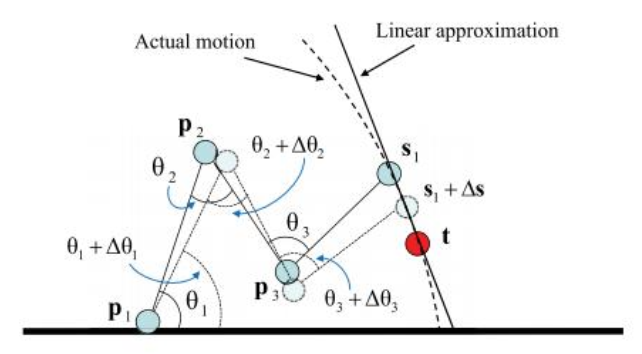
\includegraphics[width = 2.5in]{chapters/motion_matching/images/jacobian_based.png}
    \caption{Jacobian based IK solving(approximation of the first derivative)}
    \label{fig:jacobian_based}
\end{figure}

Cyclic Coordinate Descent (CCD) simplifies the IK problem by iteratively adjusting one joint at a time, minimizing the distance between the end-effector and the target\ref{fig:ccdik}. CCD is computationally efficient and easy to implement, making it popular in game engines. However, its greedy approach can lead to suboptimal solutions, especially in highly constrained scenarios.

\begin{figure}
  \centering 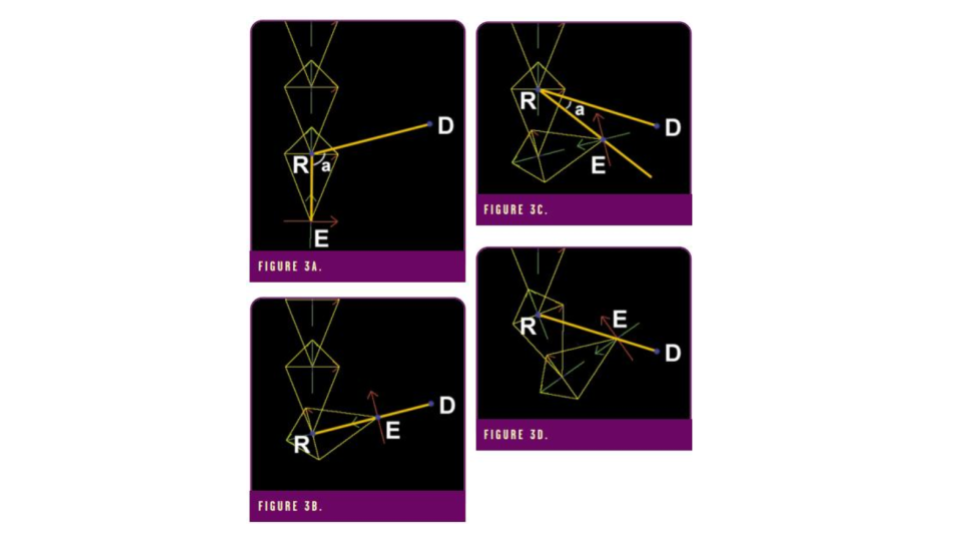
\includegraphics[width = 2.5in]{chapters/motion_matching/images/ccdik.png}
  \caption{Cyclic Coordinate Descent (CCD) IK solving(changes rotation of a joint - one at a time)}
  \label{fig:ccdik}
\end{figure}

FABRIK differs from other methods by focusing on the positions of joints rather than their angles. It iteratively adjusts the positions of joints through a two-pass approach, first from the end-effector to the root and then from the root to the end-effector\ref{fig:fabrik}. This method is known for its simplicity and stability, particularly in scenarios where maintaining a natural joint configuration is crucial.

\begin{figure}
  \centering 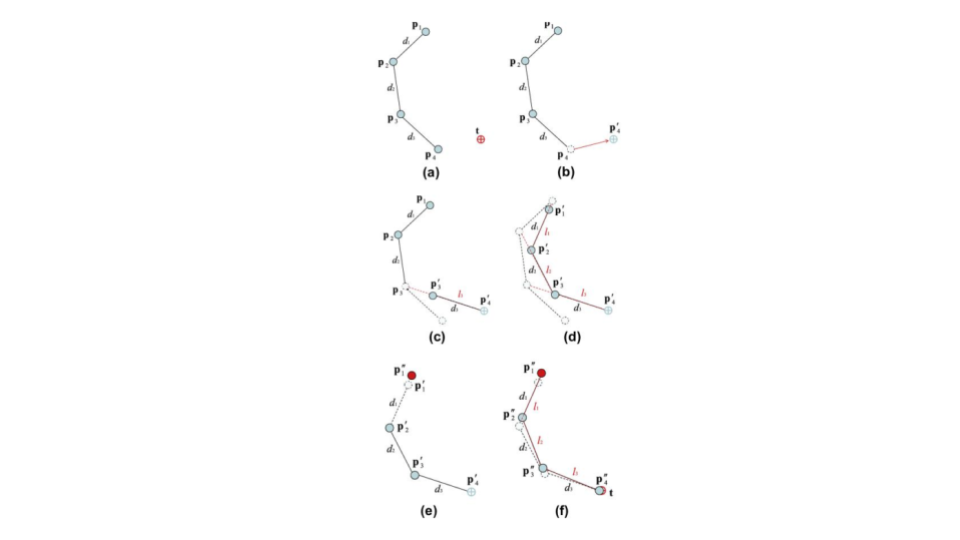
\includegraphics[width = 2.5in]{chapters/motion_matching/images/fabrik.png}
  \caption{Forward And Backward Reaching Inverse Kinematics(FABRIK) solving(updates coordinates in 2 passes)}
  \label{fig:fabrik}
\end{figure}

These classical methods have been widely adopted due to their balance between computational efficiency and control, making them suitable for a variety of real-time applications. However, they have notable limitations. They are prone to singularities, where solutions become unstable, and often require significant computational resources, especially in complex or high-dimensional systems. The resulting movements can sometimes be unnatural or biomechanically unrealistic, particularly when handling joint limits or multiple end-effectors. Additionally, these methods struggle with complex constraints and often produce suboptimal solutions that may not adapt well to varying scenarios, making them less suitable for dynamic or highly detailed applications \ref{fig:problems_classical}.

\begin{figure}
  \centering 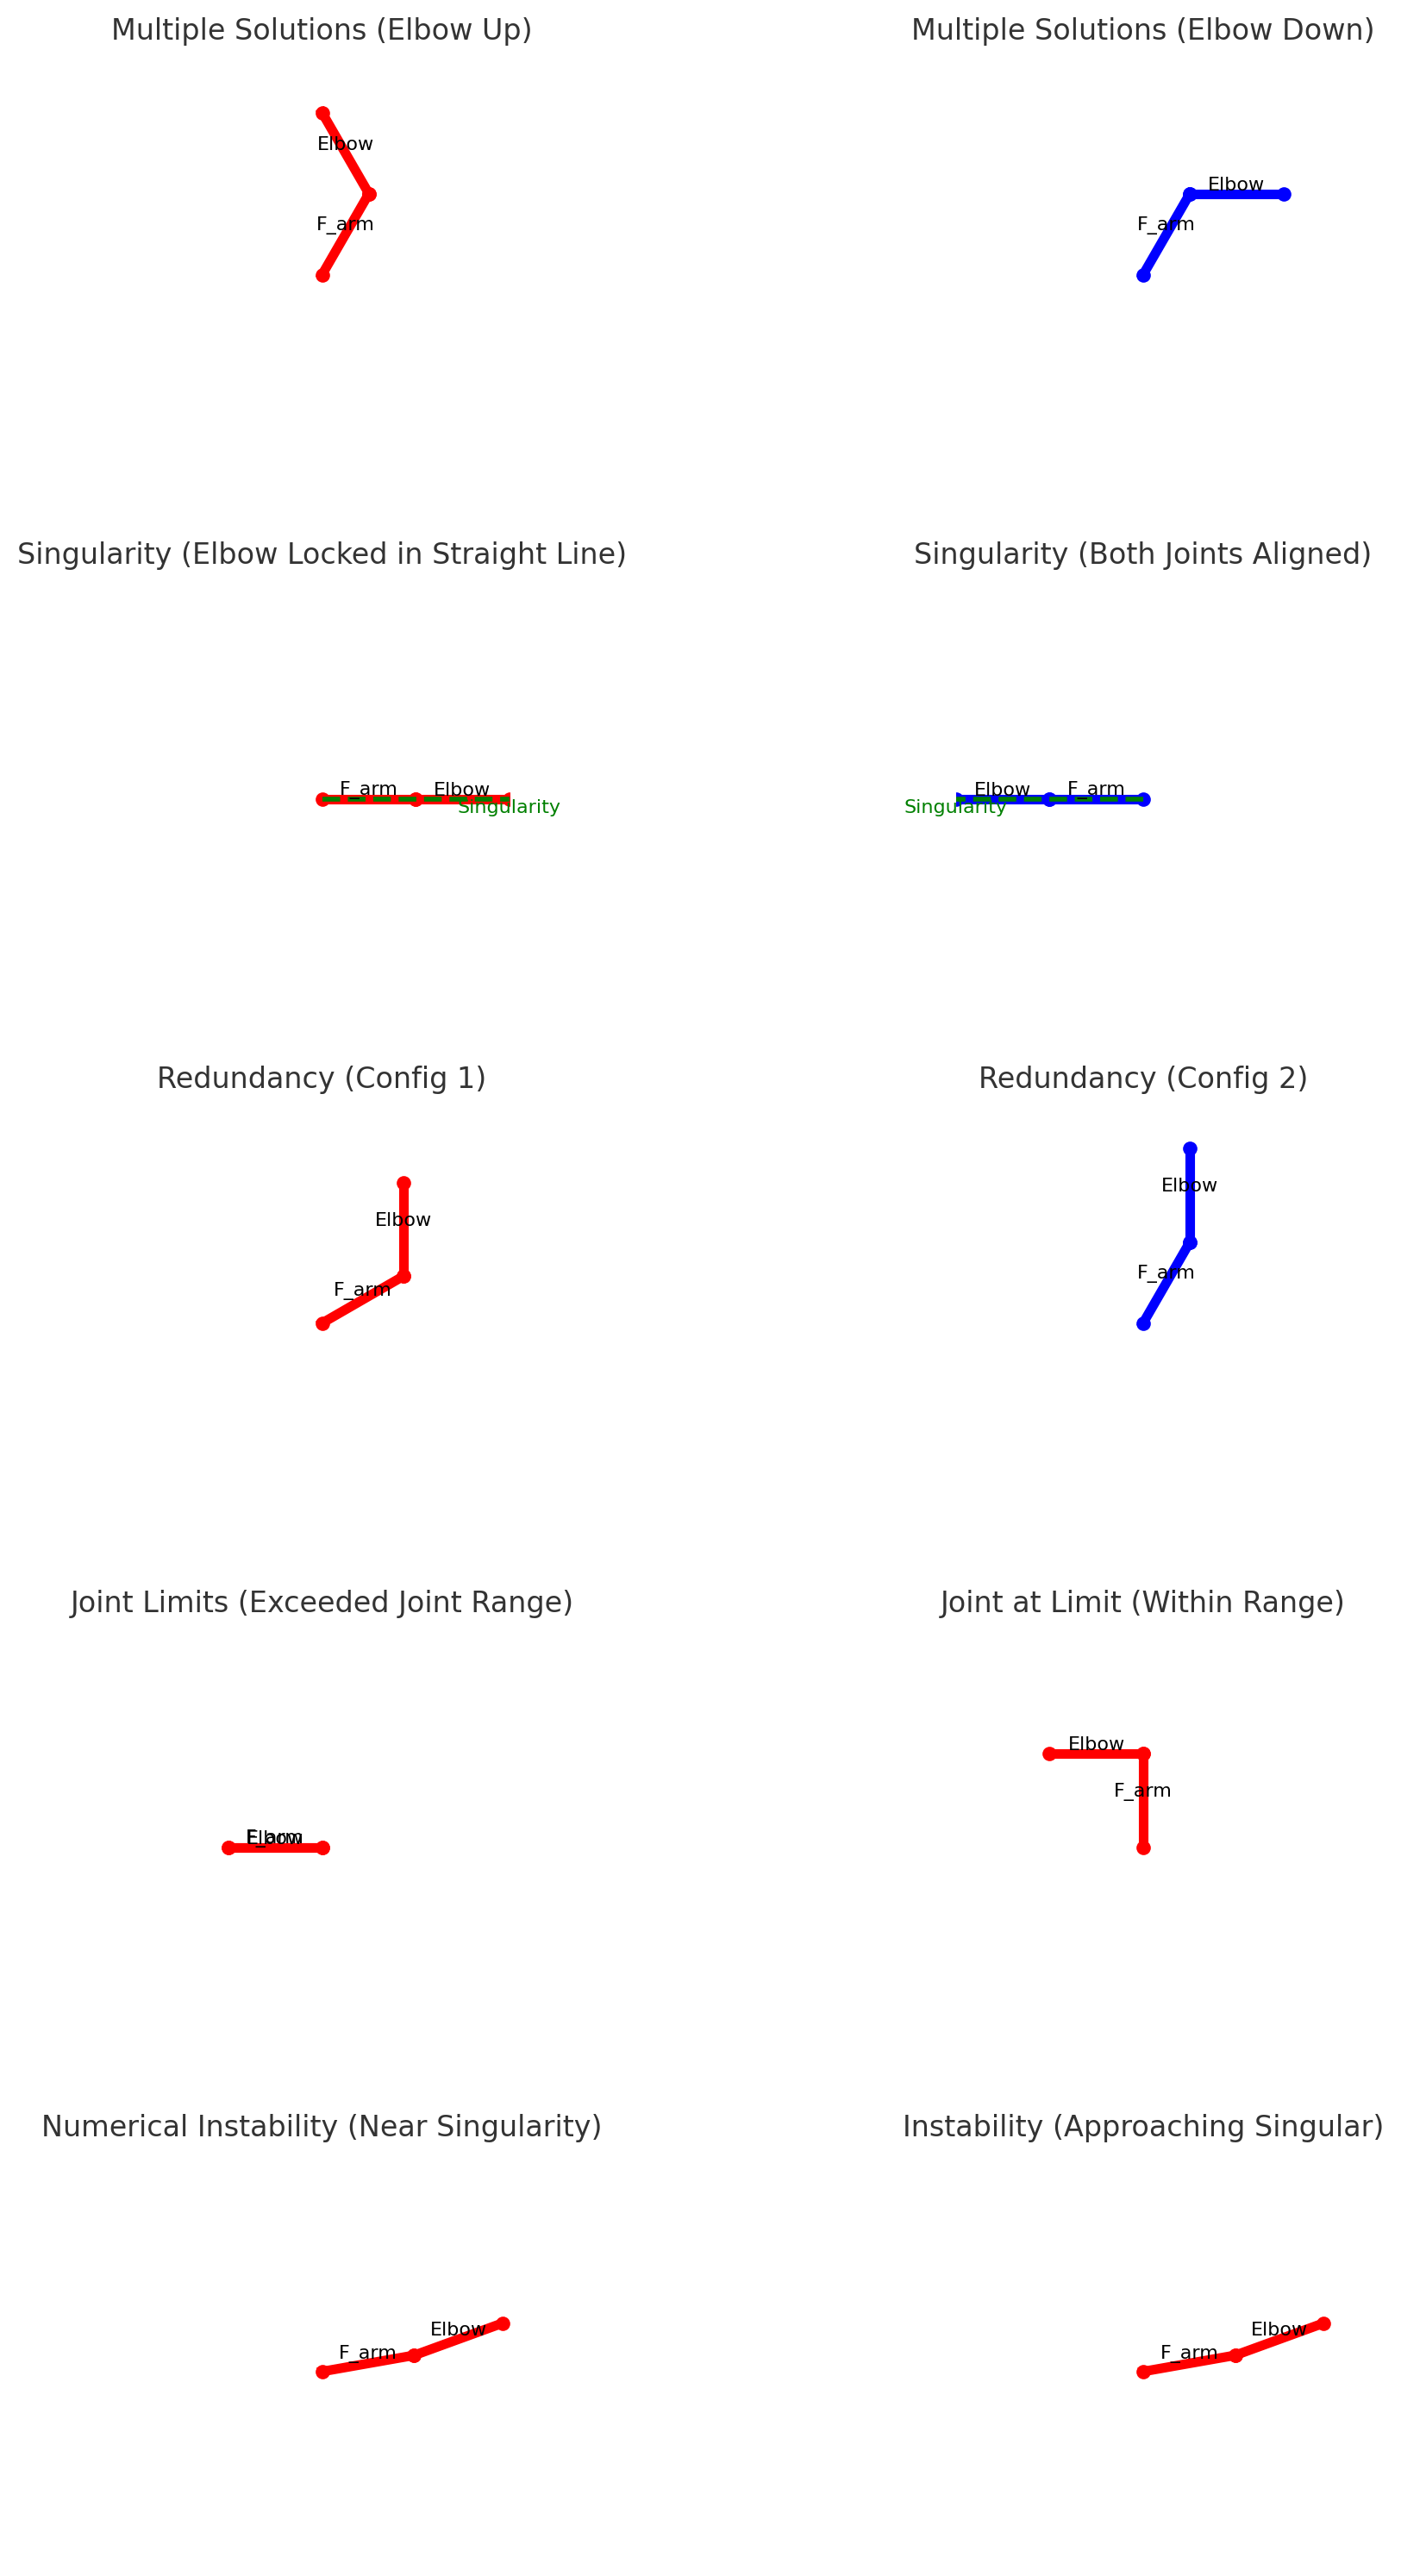
\includegraphics[width = 2.5in]{chapters/motion_matching/images/problems_classical.png}
  \caption{Problems with classical IK solving methods}
  \label{fig:problems_classical}
\end{figure}

\subsection{Data-Driven IK Approaches}
\label{ch:motion_matching:related_work:data_driven_ik}

The limitations of classical IK methods have spurred the development of data-driven approaches, which leverage large datasets and machine learning to improve the realism and flexibility of character animations.

Motion Matching represents a significant shift from traditional IK by utilizing a large database of motion capture (mocap) data. Instead of predefined animation clips, Motion Matching dynamically selects the most appropriate pose based on user inputs and contextual parameters. This approach was notably employed by Ubisoft in the game For Honor, where it enabled more fluid and responsive character animations\ref{fig:for_honor}. Motion Matching's ability to break down animations into fine-grained clips allows for seamless transitions and more natural movements.

\begin{figure}
  \centering 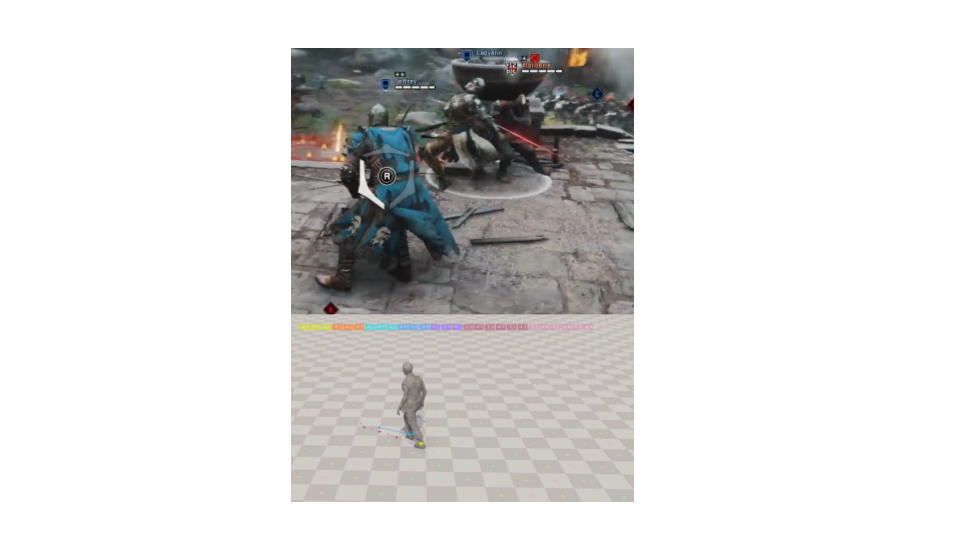
\includegraphics[width = 2.5in]{chapters/motion_matching/images/for_honor.png}
  \caption{Motion Matching in For Honor}
  \label{fig:for_honor}
\end{figure}

Phase-Functioned Neural Networks (PFNN) \cite{10.1145/3072959.3073663} (figure \ref{fig:pfnn})  extends the capabilities of motion matching by incorporating phase information into the neural network's weights. This phase-aware approach allows the network to generate contextually appropriate animations that account for the cyclical nature of bipedal movement, such as walking or running. Unlike traditional methods that rely on blending animation clips, PFNN encodes the entire animation process within the neural network, offering greater flexibility and control.

\begin{figure}
  \centering 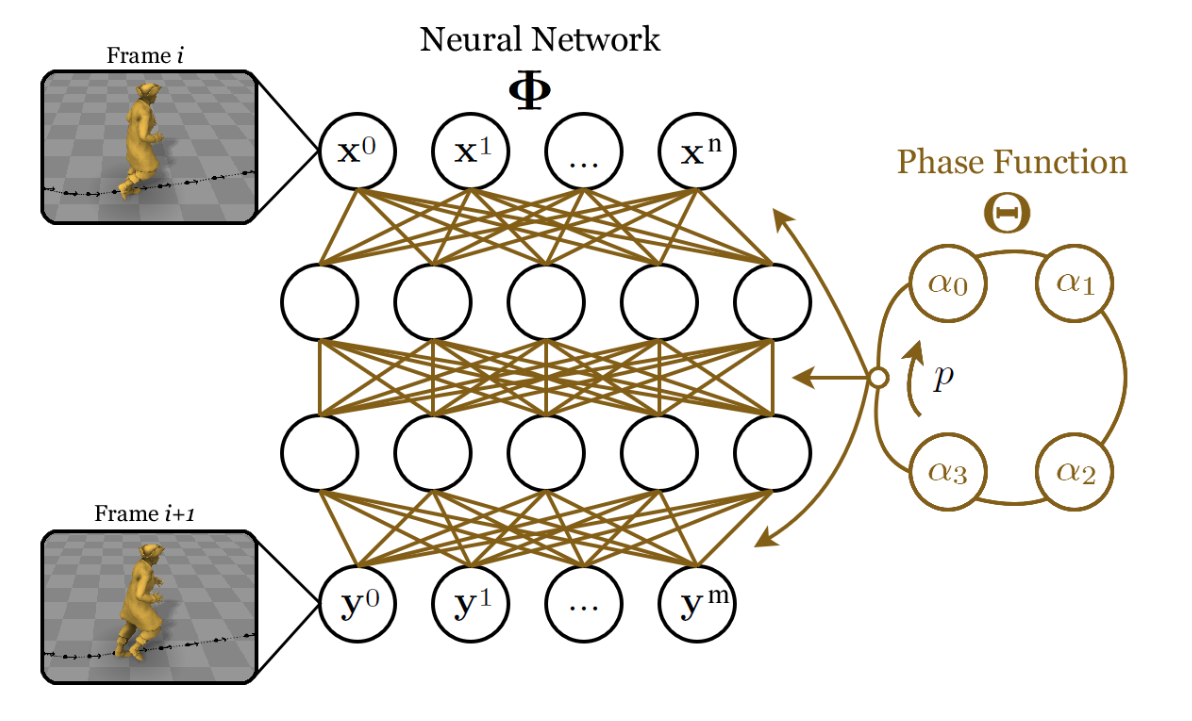
\includegraphics[width = 2.5in]{chapters/motion_matching/images/pfnn.png}
  \caption{Phase-Functioned Neural Networks (PFNN) for motion matching}
  \label{fig:pfnn}
\end{figure}

Style-Based Inverse Kinematics (Style IK) (figure \ref{fig:style_ik}) leverages machine learning to represent poses in a latent space, where the distribution of poses can be learned and sampled. Using Scaled Gaussian Process Latent Variable Models (SGPLVM), Style IK can generate stylized animations that conform to specific aesthetic or functional constraints. This approach is particularly useful for creating animations that need to adhere to a particular style or where mocap data is not available\cite{grochow2004style}.

\begin{figure}
  \centering 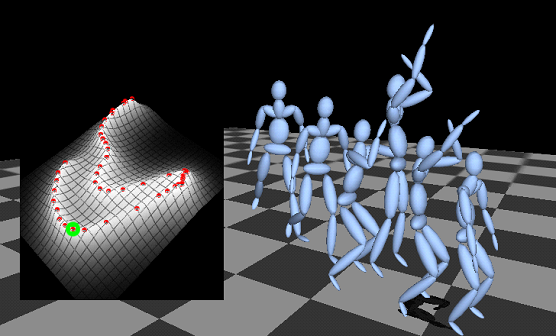
\includegraphics[width = 2.5in]{chapters/motion_matching/images/style_ik.png}
  \caption{Pose in latent space using Style IK}
  \label{fig:style_ik}
\end{figure}

These data-driven approaches represent a significant advancement over classical IK methods, offering greater flexibility, realism, and the ability to handle complex, non-linear constraints. However, they also introduce new challenges, such as the need for extensive training data and increased computational demands, particularly in real-time applications.

\subsection{Latent Space Representations in Animation}
\label{ch:motion_matching:related_work:latent_space}

Latent space representations have become increasingly important in character animation, providing a powerful tool for managing the complexity of pose and motion data. Variational Autoencoders (VAEs)\cite{kingma2013auto}, such as the one used in SMPLify-X\cite{pavlakos2019expressive}, learn a probabilistic model of human poses, allowing for the generation and manipulation of poses in a lower-dimensional space. In the context of pose estimation, VAEs help in predicting 3D poses from 2D images by learning a latent space that captures the distribution of plausible human poses. This latent space can then be sampled to generate realistic poses that meet specific constraints, such as end-effector positions or overall body posture\ref{fig:simplifyx}.

\begin{figure}
  \centering 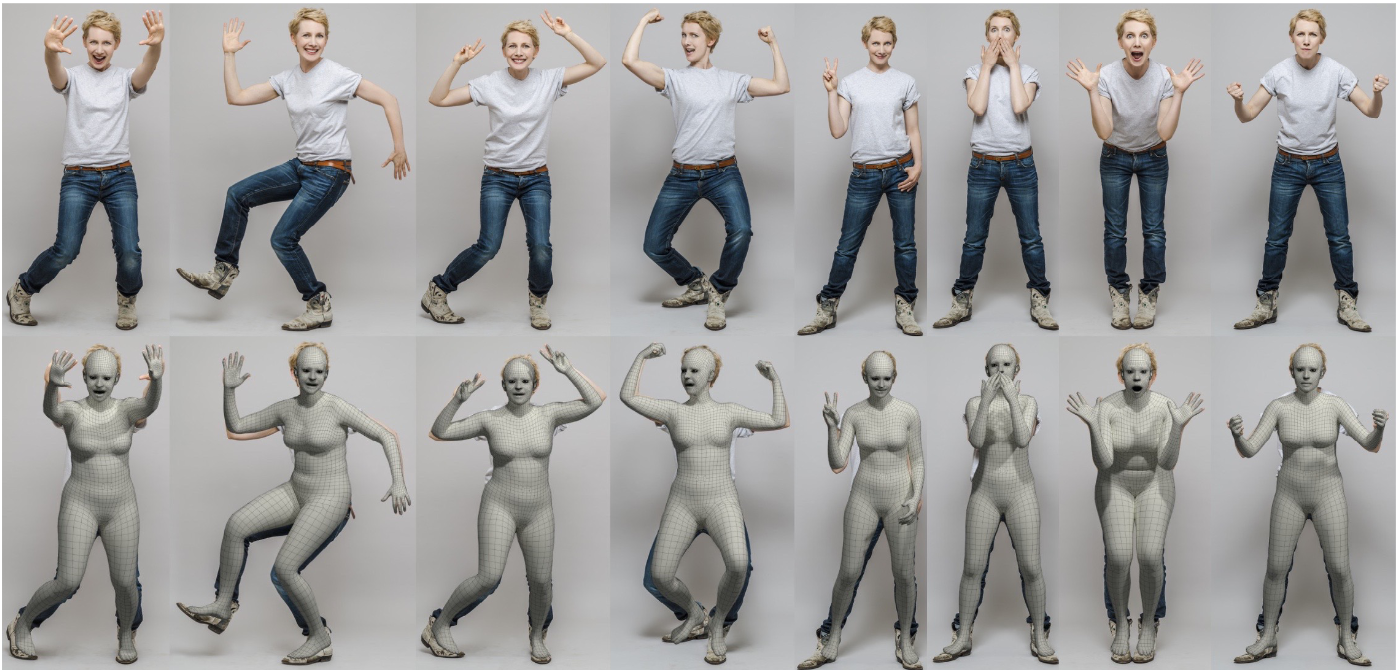
\includegraphics[width = 2.5in]{chapters/motion_matching/images/simplifyx.png}
  \caption{SMPLify-X}
  \label{fig:simplifyx}
\end{figure}

The use of latent space not only reduces the dimensionality of the data, making it easier to work with, but also enables more sophisticated manipulations, such as style transfer or the synthesis of new poses that blend characteristics from multiple examples. This has proven particularly valuable in scenarios where high-quality mocap data is not available, or where the goal is to create stylized or non-standard animations.

VPoser\cite{pavlakos2019expressive}, a specific implementation of a VAE, further demonstrates the power of latent space in animation. By encoding poses into a low-dimensional latent space, VPoser can be used in optimization processes to ensure that generated poses are both realistic and meet specific criteria. This approach is particularly effective in applications like pose estimation from monocular images, where the latent space helps to regularize the solution and avoid physically implausible poses.

Overall, latent space representations have become a crucial component of modern character animation, enabling more complex and realistic animations while also providing tools for creative control and manipulation.

\section{Motion Matching with AZee Low Level synthesis}
\label{ch:motion_matching:motion_matching_with_azee}

In this section, we discuss the application of motion matching techniques to the AZee low-level synthesis system. By integrating motion matching, data-driven IK, and latent space representations into the AZee framework, we aim to enhance the realism and expressiveness of sign language animations.

\subsection{Preparing the dataset}
\label{ch:motion_matching:motion_matching_with_azee:dataset}

The first step in integrating motion matching into AZee is to train a Variational Autoencoder (VAE) on set of sign language poses. For this task, we use a dataset of mocap data collected from the Rosetta dataset \cite{bertin2022rosetta}. The dataset consists of todo poses and should capture the diversity of poses and movements associated with different signs, providing a rich source of training data for the VAE.. Since our focus was only on the upper body, we didn't use the facial bones and the lower body for the training. We also retargeted the mocap data to the BAZeel avatar, which is compatible with the AZee skeleton structure (figure \ref{fig:retargeted}).

\begin{figure}
  \centering 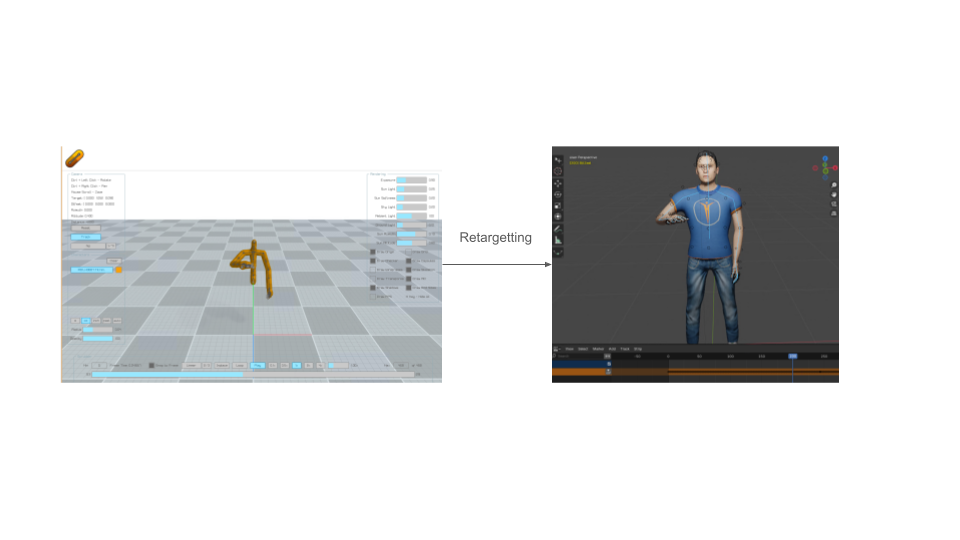
\includegraphics[width = 2.5in]{chapters/motion_matching/images/retargeted.png}
  \caption{Retargeted mocap data to BAZeel avatar}
  \label{fig:retargeted}
\end{figure}

Next, we converted the motion into AZee's FK pose array. The FK pose array consists of the rotation values of each joint in the AZee skeleton (figure \ref{fig:azee_fk_pose}). This representation is more suitable for the VAE training process, as it captures the pose information in a compact and standardized format.

\begin{figure}
  \centering 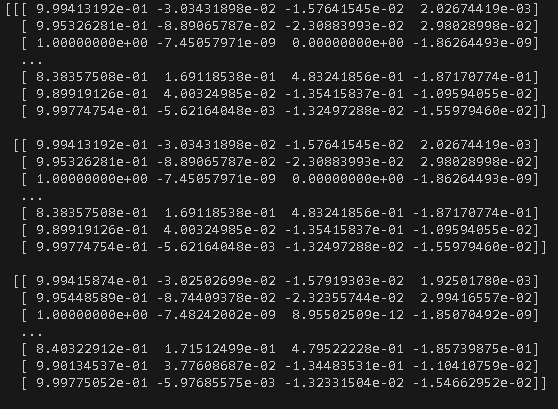
\includegraphics[width = 2.5in]{chapters/motion_matching/images/azee_fk_pose.png}
  \caption{AZee FK Pose Array}
  \label{fig:azee_fk_pose}
\end{figure}

\subsection{Training VPoser}
\label{ch:motion_matching:motion_matching_with_azee:training}

A VAE is a type of generative model that learns a low-dimensional latent space representation of the input data. In the context of character animation, a VAE can be used to capture the distribution of poses in a dataset, allowing for the generation of new poses that are statistically similar to the training data. The VAE consists of an encoder network that maps input poses to a latent space and a decoder network that reconstructs the input poses from the latent space (figure \ref{fig:vae}).

\begin{figure}
  \centering \includegraphics[width = 2.5in]{chapters/motion_matching/images/vae.png}
  \caption{Variational Autoencoder (VAE)}
  \label{fig:vae}
\end{figure}

VPoser is a specific implementation of a VAE designed for pose estimation and synthesis. We train the VPoser using the AZee FK pose array data. The training ...todo

\subsection{Implementing Motion Matching}
\label{ch:motion_matching:motion_matching_with_azee:implementation}

With the VAE trained, we can now implement a motion matching system that leverages the learned latent space to match poses generated by the AZee system to the most appropriate pose in the dataset (figure \ref{fig:motion_matching}).

\begin{figure}
  \centering \includegraphics[width = 2.5in]{chapters/motion_matching/images/motion_matching.png}
  \caption{Motion Matching with VAE}
  \label{fig:motion_matching}
\end{figure}

Algorithm \ref{alg:motion_matching} outlines the motion matching process. Given a target pose generated by the AZee synthesizor, we first encode the pose into the latent space using the VPoser encoder. We then compute the distance between the encoded pose and each pose in the dataset, selecting the pose with the smallest distance as the best match. Finally, we decode the matched pose back into the AZee FK pose array and apply it to the character.

\begin{algorithm}
  \caption{AZee constraint optimization with motion matching algorithm}
  \label{alg:motion_matching}
  \begin{algorithmic}[1]
  \For{$frame$ \textbf{in} frames}
      \State \texttt{switch\_cursor\_to\_frame($f$)}
      \For{\texttt{parallel\_block \textbf{in} self.parallel\_blocks}}
          \State \texttt{constraints.add(parallel\_block.constraints)}
      \EndFor
      \For{\texttt{constraint \textbf{in} constraints}}
          \State \texttt{constraint.apply($frame$)}
      \EndFor
      \State \texttt{model.pose\_embedding}
      \State \texttt{model.global\_trans}
      \State \texttt{optimizer = \dots}
      \For{\texttt{epoch \textbf{in} range(max\_epochs)}}
          \State \texttt{optimizer.zero\_grad()}
          \State \texttt{\dots}
          \State \texttt{optimizer.step()}
          \If{\texttt{loss.item() < threshold}} \State \texttt{break} \EndIf
      \EndFor
      \State \texttt{posture.keyframe($frame$)}
  \EndFor
  \end{algorithmic}
  \end{algorithm}

\subsection{Results and Evaluation}
\label{ch:motion_matching:motion_matching_with_azee:results}

Snapshots with standard synthesis and motion matching synthesis and the corresponding AZee code for the same are shown in table \ref{tab:results}.

\begin{table}
  \centering
  \begin{tabular}{|c|c|c|}
    \hline
    \textbf{Standard Synthesis} & \textbf{Motion Matching Synthesis} & \textbf{AZee Code} \\
    \hline
    \includegraphics[width = 1.5in]{chapters/motion_matching/images/standard_synthesis.png} & \includegraphics[width = 1.5in]{chapters/motion_matching/images/motion_matching_synthesis.png} & \begin{lstlisting}
      AZeePose pose = AZeeSynthesize();
      AZeeMotionMatch(pose);
    \end{lstlisting} \\
    \hline
  \end{tabular}
  \caption{Results of Motion Matching Synthesis}
  \label{tab:results}
\end{table}

The synthesized videos can also be viewed at \href{todo}.

todo compared to cmu based poser.

Initial subjective evaluations suggest that the motion matching system produces more natural and contextually appropriate animations compared to standard synthesis. However, due to the lack of good quality mocap data, the integration of motin matching into Sign Language synthesis is still in the early stages. We also observe that the system can change the pose of the character in a way that is not always desirable \ref{fig:problem_motion_matching}.

\begin{figure}
  \centering \includegraphics[width = 2.5in]{chapters/motion_matching/images/problem_motion_matching.png}
  \caption{Problems with motion matching}
  \label{fig:problem_motion_matching}
\end{figure}

Lastly, figure \ref{fig:losses} shows how retargeting the mocap data to the AZee skeleton structure results in a loss of information. This loss can affect the quality of the generated animations and is an area for future improvement.

\begin{figure}
  \centering 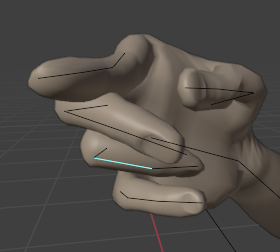
\includegraphics[width = 2.5in]{chapters/motion_matching/images/losses.png}
  \caption{Losses in retargeting mocap data}
  \label{fig:losses}
\end{figure}

\section{Discussion}
\label{ch:motion_matching:discussion}

The integration of motion matching into the AZee system represents a significant advancement in sign language synthesis. By leveraging data-driven IK and latent space representations, we are able to generate more realistic and contextually appropriate sign language animations. This has the potential to enhance the expressiveness and naturalness of sign language avatars, making them more engaging and accessible to users. In some ways, this offfers a new perspective to Sign Language synthesis where the linguistics decides the "what" and the motion matching decides the "how" of the animation.

For future, posers based on neural distance fields \cite{tiwari2022pose} or diffusion \cite{lu2023dposer} could be used for motion matching since the current poser has a bayesian bias. Also, continuity of motion matching with respect to signing spaces could be studied further improving the the learnt pose prior.

While the integration of machine learning into SL synthesis offers numerous advantages, it also introduces new challenges. Data-driven and latent space methods typically require significant computational resources, both during training and inference. This can be a major barrier in real-time applications, where low latency is critical. Also the effectiveness of machine learning models depends heavily on the availability of high-quality training data. In many cases, obtaining sufficient mocap data can be difficult, especially for non-standard or stylized animations. Lastly, while machine learning models can generate realistic and high-quality animations, they often lack the fine-grained control that human animators require. Ensuring that these models produce outputs that align with artistic vision remains a significant challenge.

\end{document}